%
% Main thesis LaTeX file. We use the REPORT style format
% instead of article for most technical papers
%
%
\documentclass[12pt,fleqn]{article}

%%%%%%%%%%%%%%%%%%%%%%%%%%%%%%%%%%%%%%%%%%%%%%%%%%%%%%%%%%%%%%%%%%%%
%
% list the set of packages we use for various aspects of 
% the thesis format
%
\usepackage{layout}
\usepackage[utf8]{inputenc}
\usepackage{setspace}

\usepackage{tabularx}
\usepackage{subfigure}
\usepackage{epsfig}
\usepackage{float}
\usepackage{floatflt}
\usepackage{listings}
\usepackage{palatino}
\usepackage{verbatim}
\usepackage{footnpag}
\usepackage{caption}
\usepackage[mathcal, mathbf]{euler}
\usepackage{amsmath}
\usepackage{amstext}
\usepackage{color}
\usepackage{xcolor}
\usepackage{graphicx}


%%%%%%%%%%%%%%%%%%%%%%%%%%%%%%%%%%%%%%%%%%%%%%%%%%%%%%%%%%%%%%%%%%%%
%
% include two local LaTeX source files that establish the
% thesis layout and the set of additional commands we find
% useful for creating the text.
%
\input{layout}
\input{newcommands}
\input{outline_support}


\newcommand{\Organization}{School of Computer Engineering}

\title{CE3001 Lab3. Simple Control and Datapath}

\author{
  Lu Shengliang \\
  SLU001\\
  \Organization{} \\
  \vspace*{-10mm} \\
  Nanyang Technological University \\
  \vspace*{-10mm} \\
  SLU001@e.ntu.edu.sg
}

%
% This begins the actual lab report
%
\renewcommand{\OutlineLevel}{2}

\begin{document}

\maketitle

\begin{abstract}
\ls{1}
\textbf{Simple Control} and \textbf{Datapath} are designed to implement indirectly feeding data inputs to ALU or RF. It is required to perform a sequence of operations by employing an control unit.
\ls{1.2}
\end{abstract}

\ls{1.2}


\section{Introduction}

\label{sec:intro}

%=====================================================================
\subsection{Control Unit \& Datapath Specification} 
The ADD, SUB, AND and OR instructions have a three address format(Table 1).
opCode $R_d$, $R_s$, $R_t$ (Execution is \ensuremath{R_d \Rightarrow R_s} (OP) $R_t$). $R_d$ is the destination register, and $R_s$ and $R_t$ are the source registers for operand 1 and 2, respectively. The bit-level format for the three-address format is:
\begin{table}
  \centering
  \begin{tabularx}{\textwidth}{| X | X | X | X | X |}
    \hline
    \textbf{} & \textbf{opCode} & \textbf{$R_d$} & \textbf{$R_s$} & \textbf{$R_t$}\\ \hline
    \textbf{Index} & 15-12 & 11-8 & 7-4 & 3-0 \\
    \hline
  \end{tabularx}
  \caption{Instruction Format 1}
\end{table}

The SLL, SRL, SRA, and RL instructions have a two address and one immediate format.
opcode $R_d$, $R_s$, imm (Execution is \ensuremath{R_d \Leftarrow R_s} (OP) imm). $R_d$ is the destination register, $R_s$ is the source register and imm is used as the shift amount for ALU. The bit-level format for the two address plus immediate format is:
\begin{table}
  \centering
  \begin{tabularx}{\textwidth}{| X | X | X | X | X |}
    \hline
    \textbf{} & \textbf{opCode} & \textbf{$R_d$} & \textbf{$R_s$} & \textbf{imm}\\ \hline
    \textbf{Index} & 15-12 & 11-8 & 7-4 & 3-0 \\
    \hline
  \end{tabularx}
  \caption{Instruction Format 2}
\end{table}

\subsection{Design structure \& Port list}
A block diagram of the expected design is shown in Figure 1.

\begin{figure}[H]
\centering
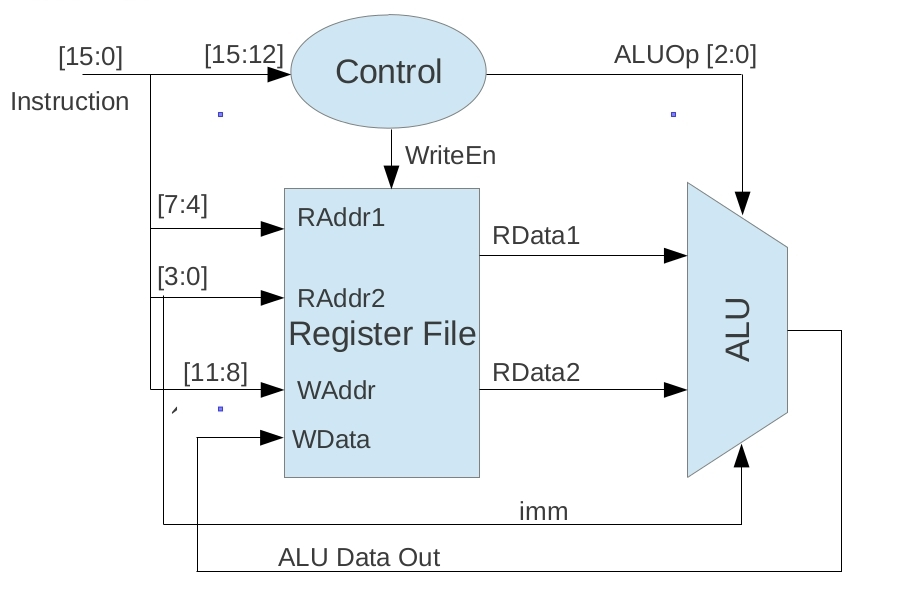
\includegraphics[width=\textwidth]{controlUnit.jpg}
\caption{Control Unit and Datapath}
\end{figure}

And the port name are listed below.

\begin{table}
  \centering
  \begin{tabular}{| l | l | l | l |}
    \hline
    \textbf{Port Name} & \textbf{Direction} & \textbf{Size} & \textbf{Description}\\ \hline
    Instruction & Input & 16 bit & Instruction word \\
    \hline
    DataInit & Input & 16 bit & Initialization Data \\
    \hline
    InitSel & Input & 1 bit & Select bit from Initialization data \\
    \hline
    AlUOut & Output & 16 bit & Data Output from the ALU \\
    \hline
  \end{tabular}
  \caption{Port List Specification}
\end{table}


%=====================================================================
\subsection{Structure of the rest of the paper}
The rest of the paper first describes the Verilog implementation of \textbf{Control Unit} and \textbf{Datapath} in \emph{Section \ref{sec:impl}}. \emph{Section \ref{sec:eval}} presents the experimental results using \emph{testbench}, which valid the functionality of our RF. \emph{Section \ref{sec:concl}} presents our conclusions and discussions.
%=====================================================================


\section{Implementation}
\label{sec:impl}

%=====================================================================

\subsection{Verilog Code Control.v}
\lstset {
    language=Verilog,
    backgroundcolor=\color{black!5},
    basicstyle=\ttfamily\footnotesize,
    numbers=left,
    numberstyle=\tiny,
    frame=single
}
\renewcommand{\baselinestretch}{0.75}
\begin{lstlisting}
module Control (input [3:0] ControlInput, output WriteEn, ALUop);
  assign WriteEn = ControlInput[3];
  assign ALUop = ControlInput[2:0];
endmodule
\end{lstlisting}
\end{\baselinestretch}
Our implementing strategies are using concatenation, which are basic assignments.\\
The related testbench implementation results will be listed in \emph{Section \ref{sec:eval}}.

%====================================
\subsection{Verilog Code datapath.v}
\lstset {
    language=Verilog,
    backgroundcolor=\color{black!5},
    basicstyle=\ttfamily\footnotesize,
    numbers=left,
    numberstyle=\tiny,
    frame=single
}
\renewcommand{\baselinestretch}{0.75}
\begin{lstlisting}
module datapath(input [15:0] Instruction, DataInit,
                input InitSel, input clk, reset,
                output [15:0] ALUOut);

  wire [15:0] WData;
  wire [15:0] RData1, RData2;
  wire [3:0] RAddr1, RAddr2, WAddr;
  wire [2:0] ALUop;
  wire Wen;
  
  assign  RAddr1 = Instruction[7:4];
  assign  RAddr2 = Instruction[3:0];
  assign  WAddr = Instruction[11:8];
  assign  WData = InitSel ? ALUOut : DataInit;
  
  Control Con(.ControlInput(Instruction[15:12]),
              .WriteEn(Wen), .ALUop(ALUop));
  Reg_File Reg(.RAddr1(RAddr1), .RAddr2(RAddr2),
               .WAddr(WAddr), .WData(WData),
               .Wen(Wen), .Clock(clk), .Reset(reset),
               .RData1(RData1), .RData2(RData2)); 
  alu a0(.A(RData1), .B(RData2), .op(ALUop),
         .out(ALUOut), .imm(RAddr2));
endmodule
\end{lstlisting}
\end{\baselinestretch}
The datapath module is used to manage the \emph{Datapath} for ALU, RF and control Unit. It takes the instruction input and separate it to different ports.\\


\section{Evaluation}
\label{sec:eval}

%=====================================================================
\subsection{Testbench Code Control\underline{ }tb.v}
\lstset {
    language=Verilog,
    backgroundcolor=\color{black!5},
    basicstyle=\ttfamily\footnotesize,
    numbers=left,
    numberstyle=\tiny,
    frame=single
}
\renewcommand{\baselinestretch}{0.75}
\begin{lstlisting}
module Control_tb();
  reg [3:0] control_input;
  wire WriteEn;
  wire [2:0] ALUOp;
  
  Control C0(
             control_input,
             WriteEn,
             ALUOp
             );
  
  initial
    begin
      control_input = 0;
      #10 control_input = 4'b1010;
      #10 control_input = 4'b1100;
      repeat (10) begin
       #10 control_input = $random;
      end
      #10 $finish;
    end
endmodule // Control_tb
\end{lstlisting}
\end{\baselinestretch}
A testbench has been designed to test the \emph{Control.v} file. A simulation function is provided by \emph{ModelSim} software. 
\begin{figure}[H]
\centering
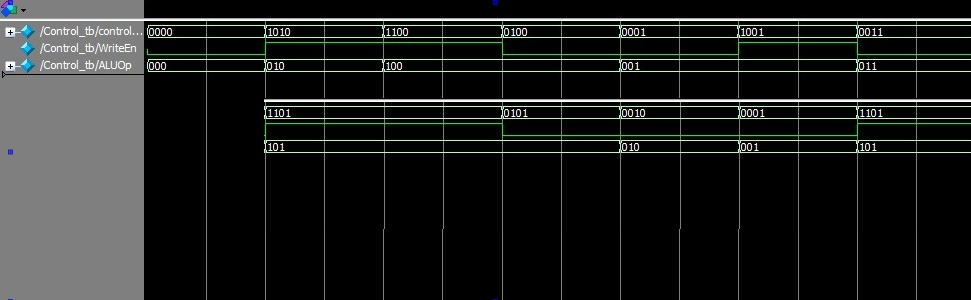
\includegraphics[width=\textwidth]{control_tb.jpg}
\caption{Control\underline{ }tb results}
\end{figure}
%=================================================================
\subsection{First Testbench Code datapath\underline{ }tb.v}
\lstset {
    language=Verilog,
    backgroundcolor=\color{black!5},
    basicstyle=\ttfamily\footnotesize,
    numbers=left,
    numberstyle=\tiny,
    frame=single
}
\renewcommand{\baselinestretch}{0.75}
\begin{lstlisting}
module dataPath_tb();
  reg [15:0] Instruction, DataInit;
  reg InitSel, clk, reset;
  wire [15:0] ALUOut;
  datapath dp1(.Instruction(Instruction),
                     .DataInit(DataInit),
                     .InitSel(InitSel),
                     .clk(clk),
                     .reset(reset),
                     .ALUOut(ALUOut)
                     );
  always #5 clk = ~clk;
  initial begin
    reset = 0;
    clk = 0;
    #20 reset = 1;
    repeat (10000) begin
      #10 InitSel = 0;
      {DataInit, Instruction} = $random;
    end
    repeat (15) begin
      {Instruction, DataInit} = $random;
      InitSel = $random;
      #10 $display("Instruction = %b, ALUOut = %b",
                    Instruction, ALUOut);
    end
    $finish;
  end // initial begin
endmodule // dataPath_tb
\end{lstlisting}
\end{\baselinestretch}
The testbench firstly ran 10000 times randomly write initial data in to RF(we assumed 10000 should be enough. and actually it did), to make sure RF are full of data rather than \emph{xxxx xxxx}.\\
Then there were 15 times randomly testing cases, in order to test ALUOut connection with RF, Control and datapath modules.\\
There is one more testbench provided by lecturer, which will be given below.

\subsection{Second Testbench Code datapath\underline{ }tb\underline{ }file\underline{ }io.v}
\lstset {
    language=Verilog,
    backgroundcolor=\color{black!5},
    basicstyle=\ttfamily\footnotesize,
    numbers=left,
    numberstyle=\tiny,
    frame=single
}
\renewcommand{\baselinestretch}{0.75}
\begin{lstlisting}
`include "datapath.v"
`timescale 1ns / 10ps
`define EOF 32'hFFFF_FFFF
`define NULL 0
`define MAX_LINE_LENGTH 1000
`define ISIZE 16
`define DSIZE 16
module datapath_tb_fileio;
  reg                        clk_half;
  reg                        clk;
  reg                        rst;
  reg                        InitSel;
  reg [`ISIZE-1:0]           Instruction;
  reg [`DSIZE-1:0]           DataInit;
  integer                    file_input, file_output;
  integer                    file_gold, c, r;
  reg [15:0]                 exp;
  reg [8*`MAX_LINE_LENGTH:0] line;
  wire [`DSIZE-1:0]          ALUOut;
  datapath datapath_inst (
                          .clk(clk),
                          .reset(rst),
                          .Instruction(Instruction),
                          .InitSel(InitSel),
                          .DataInit(DataInit),		                      
                          .ALUOut(ALUOut)
                          );
  always #5 clk = ~clk;
  always@(posedge clk)
    clk_half <= ~clk_half;
  initial
    begin
      file_input  = $fopen("input.txt","r");
      file_output = $fopen("output.txt","w");
      file_gold   = $fopen("gold.txt","r");
      clk = 0;
      clk_half =0;
      rst = 1;
      #5 rst = 0;
      #10 rst = 1;
      InitSel = 0;
      while (!$feof(file_input))
        begin
          c = $fgetc(file_input);
          if (c == "/" | c == "#" | c == "%")
            r = $fgets(line, file_input);
          else
            begin
              r = $ungetc(c, file_input);
              r = $fscanf(file_input, "%h %h %b",
                          Instruction, DataInit, InitSel);
            end
          #20; // 20ns for each iteration
        end // while (!$feof(file_input))
      $fclose(file_input);
      $fclose(file_gold);
      $fclose(file_output);
      #100 $finish;
    end	// end of initial
  always@(posedge clk_half)
    if (InitSel)
      begin
        $fwrite(file_output, "%h\n", ALUOut);
        r = $fscanf(file_gold, "%h\n", exp);
        if (ALUOut != exp)
          begin
            $fdisplay(file_output, "Error: expected: %h\n", exp);
          end
        else
          $fdisplay(file_output, "Matched: %h", ALUOut);
      end
endmodule // datapath_tb_fileio
\end{lstlisting}
\end{\baselinestretch}
This testbench reads instruction and data from a file named \emph{input.txt}. And then, it generates the value accordingly and compares it with given correct results which given from file \emph{gold.txt}.\\

\lstset {
    language=Verilog,
    backgroundcolor=\color{black!5},
    basicstyle=\ttfamily\footnotesize,
    numbers=left,
    numberstyle=\tiny,
    frame=single
}
\renewcommand{\baselinestretch}{0.75}
\begin{lstlisting}
//===========
// input.txt|
//===========
//++++++++++++++++++++++++++++++++++++++++++++++++++++++++++++
// file_input.txt
// format:
// Instruction(hex)	DataInit(hex)	InitSel(bin)
// First, initialize the register file
8000	0010	0
8100	0011	0
8200	0012	0
8300	0013	0
8400	0014	0
8500	0015	0
8600	0016	0
8700	0017	0
8800	0018	0
8900	0019	0
8a00	001a	0
8b00	001b	0
8c00	001c	0
8d00	001d	0
8e00	001e	0
8f00	001f	0

// verify alu
8321	xxxx	1
9421	xxxx	1
a521	xxxx	1
b621	xxxx	1
c721	xxxx	1
d821	xxxx	1
e921	xxxx	1
fa21	xxxx	1

//===========
//  gold.txt|
//===========
//++++++++++++++++++++++++++++++++++++++++++++++++++++++++++++
0023
0001
0010
0013
0024
0009
0009
0024

//===========
//output.txt|
//===========
//++++++++++++++++++++++++++++++++++++++++++++++++++++++++++++
0023
Matched: 0023
0001
Matched: 0001
0010
Matched: 0010
0013
Matched: 0013
0024
Matched: 0024
0009
Matched: 0009
0009
Matched: 0009
0024
Matched: 0024
0024
Matched: 0024
\end{lstlisting}
\end{\baselinestretch}
The testbench is used to generate output and compare it with \emph{gold.txt} file. If everything is matched, then the \emph{datapath.v} itself should be correct.
\section{Conclusions and Future Work}
\label{sec:concl}
The datapath design works properly based on two sets testing results.
\\ 
%=====================================================================
%\subsection{\emph{Problems} occurred in our approach}
For this report, the testbench given has small mistake, which are supposed to be fixed.
\\
%\subsection{Available \emph{Improvement}}
The connection of different modules are complicated. It is better if we can draw the diagram out first.
%=====================================================================
\end{document}
